\chapter{Computer Science Background}
\label{ch:computerscience}

Random-walk based \ac{NRL} methods have been chosen for use in this thesis to address the shortcomings with engineered features. Learned feature vectors of nodes and edges would be generated from these methods of which the core is language model skip-gram (one type of word2vec model). Perozzi et al. ~\cite{perozzi_deepwalk:_2014} developed DeepWalk to apply random walk to network for generating walks analog to sentences for training skip-gram model. In DeepWalk, the walks (sentences) are parsed into a one-layer neural network to learn the occurrence relationships between nodes (words). Then, the weights of the neural network would be kept for generating node (word) vectors. At last, learned feature vectors of nodes can be used for downstream machine learning methods. Node2vec ~\cite{grover_node2vec:_2016} improves DeepWalk by adding in-out (p) and return (q) parameters to generate biased random walk to perform a flexible neighbourhood sampling strategy. Edge2vec ~\cite{gao_edge2vec:_2018} was improved further by applying an \ac{EM} algorithm to calculate a edge-type specific \ac{TPM} with edge semantics information. 

\section{Language Models}

Word2vec is a group of related models to produce word embeddings created by Mikolov et al.~\cite{mikolov_efficient_2013}. It gives a two-layer neural network to capture the co-occurrence of words in sentences, including two main models, continuous bag-of-word and skip-gram. Continuous bag-of-word predicts the current word from a window of surrounding context words, which is adapted for drug repositioning by Ngo et al. ~\cite{ngo_application_2016}, and the skip-gram model conversely uses the word to predict its surrounding words.

When training the neural network, every word in the training set is encoded as one-hot vector. After feeding the pairs of words to a two-layer neural network, backpropagation is applied to update the weights in the hidden layer. The training objective is to minimize the summed prediction error across all context words in the output layer. Each word is then represented by a distribution of weights across the hidden layer.

\subsection{Skip-Gram Model}

In this thesis, the skip-gram model is implemented in node2vec and edge2vec. According to Rong’s explanation to word2vec ~\cite{rong_word2vec_2014}. As illustrated in Figure \ref{fig:skip-gram}, this model takes one word as input to a log-linear classifier with continuous projection layer in order to predict the context of the word in a certain range. The training complexity is presented in Equation 2

\begin{equation}
Q=C\times(D+D\times log_{2}V)
\end{equation}

Where C is the maximum distance of the words, R in range <1,C> could be selected, R words before and after the target words are used as labels to train the neural network. In this model, there exist two vector representations for each word in the vocabulary: the input vector Vw, and the output vector Vw’. Learning the input vectors is cheap; but learning the output vectors is very expensive. Then hierarchical softmax and negative sampling are used for optimizing computational efficiency ~\cite{rong_word2vec_2014}.

Intuitively, the skip-gram model give the word vector according to its surrounding contexts, which means if two words have similar meanings or tied together often, they should have similar vectors, for example, the vector of “france” is similar to that of “canada”.

\begin{figure}[!h]
    \centering
    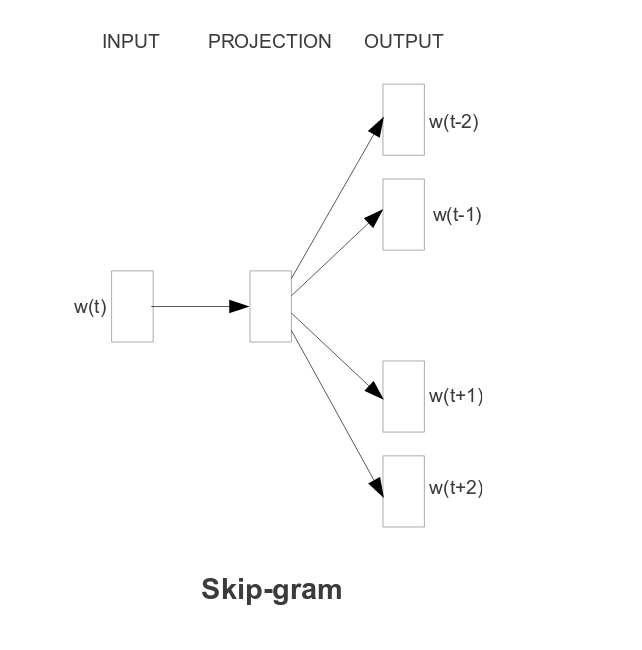
\includegraphics[scale=0.35]
    {figures/skip-gram.png}
    \captionsetup{justification=centering}
    \caption[The structure of skip-gram model]{\label{fig:skip-gram} The structure of skip-gram model. Figure adapted from ~\cite{mikolov_efficient_2013}}
\end{figure}

\section{Random Walk Based Network Representation Learning Models}

Generating random walks is a stochastic method that was first introduced by Karl Pearson in 1905 ~\cite{pearson_problem_1905}. A node w is selected from a graph as a starting point, then randomly select one of its neighbors n as next node to go. At last, the sequence of nodes selected in such way is a walk. The probability for the walk to move from w to the n is called transition probability. According to transition probability, the walk is still random but could be more or less possible to one specific node than another.

The transition probabilities contain information about the edge. If the edge e is very important, intuitively, the transition probability to go through e should be higher than many other edges around the starting node w.

\subsection{DeepWalk}

DeepWalk is from Perozzi et al. ~\cite{perozzi_deepwalk:_2014}, it uses random walk to make ‘sentences’ from network, then train the skip-gram model to get the feature vectors of nodes. The algorithm has two parts, the first one is to apply random walk and the second one is to train a skip-gram model. In the first step, the random walk generator takes network G as homogeneous and uniform, starting from vertex Vi to its neighbors until getting to the walk length t. All the walks are ‘sentences’ to skip-gram model to capture the occurrence probability of ‘words’ (nodes) in the network.

DeepWalk outperformed other previous methods like SpectralClustering ~\cite{von_luxburg_tutorial_2007}, EdgeCluster ~\cite{tang_scalable_2009}, Modularity ~\cite{tang_relational_2009}, wvRN~\cite{Macskassy_a_2003}, and Majority (This naive method simply chooses the most frequent labels in the training set) with evaluation as micro-F1 and macro-F1. Also, the parameter sensitivity was tested. For dimensionality, the level of changes of results highly depends on the dataset. The performance of the model is sensitive to the number of random walk. When the number of random walks is above 10, the results have no outstanding improvements. It suggests that a small number of random walk could learn a meaningful latent representation.

\subsection{Node2vec}

As illustrated in Figure \ref{fig:node2vec}, given a node \textit{v}, random walk would go to the neighbors \textit{x}. there are three types of neighbor: one is the previous node \texti{t}, one is neighbor \textit{$x_2$} connecting with the previous node \textit{t}, another one is \textit{$x_2$} (or \textit{$x_3$}) only connecting with \textit{v}, but not with the previous node \textit{t}.So the shortest path distances ($d_{tx}$) for \textit{t}, \textit{$x_1$}, \textit{$x_2$}, \textit{$x_3$} to \textit{t} are 0, 1, 2, 2. Transition probability $\pi$ is calculated as Equation \ref{tp_node2vec}, $w_{vx}$  is the weight of edge between node \textit{v} and \textit{x}. In Equation \ref{tp_node2vec}, \textit{p}, \textit{q} and weights are integrated in transition probability for generating walks (sentences) for skip-gram model.

\begin{equation}\label{tp_node2vec}
  \pi_{vx} =
    \begin{cases}
      \frac{1}{p} \times $w_{vx}$ & \text{if $d_{tx} = 0$}\\
      1 \times $w_{vx}$ & \text{if $d_{tx} = 1$}\\
      \frac{1}{q} \times $w_{vx}$ & \text{if $d_{tx} = 2$}
    \end{cases}       
\end{equation}

Node2vec ~\cite{grover_node2vec:_2016} is improved from DeepWalk, adding a return parameter \textit{p} and an in-out parameter \textit{q} during calculation of the node \ac{TPM}. \textit{p} is the return parameter. When \textit{p} is smaller than 1 and \textit{q}, the probability of returning $1/ p$ is bigger than 1 and $1/q$. Random walk would be more likely to go back to t  (Figure \ref{fig:node2vec}), so the walk is more local. \textit{q} is the in-out parameter. When \textit{q} is bigger than 1, the probability of going out ($1/q$) is smaller than 1, then still the walk would be more local. If \textit{q} is smaller than 1, the walk would be more global.

\begin{figure}[!h]
    \centering
    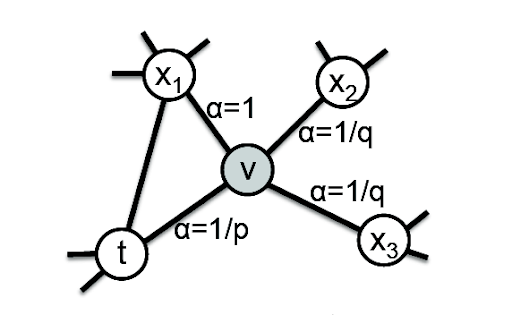
\includegraphics[scale=0.4]
    {figures/node2vec.png}
    \captionsetup{justification=centering}
    \caption[An illustration of random walk procedure in node2vec]{\label{fig:node2vec} An illustration of random walk procedure in node2vec. Figure adapted from ~\cite{grover_node2vec:_2016}}
\end{figure}

\subsection{Edge2vec}

In edge2vec algorithm, Zheng et al. ~\cite{gao_edge2vec:_2018} improved node2vec by making use of \ac{EM} algorithm to calculate an additional TPM based on edge types. Edge2vec is based on the assumption that the distribution of edges in different samples are valid estimator of transition correlation in the graph. If two edge types are highly correlated then the transition probability between them is high, and vice versa. With such method, those edge types which are less distributed in the network, but actually important would be more likely to be passed through during random walk. And then the model can capture more comprehensive information of the network.

The edge2vec algorithm contains two parts, generating \ac{TPM} with \ac{EM} algorithm and generating walks according to the \ac{TPM}. The first part starts with a transition probability matrix initiated as all the same number $1/n^2$ with a matrix size $n * n$ (n is the number of edge types in network). Expectation step is to generate walks based on the current \ac{TPM}. Usually a random walk starts from every node in the network, but in edge2vec, there is a parameter ‘max\_count’ constraining the number of starting nodes. Originally, the biggest ‘max\_count’ is 1,000. It means sampling at most 1,000 starting nodes from all nodes. And then in the Maximization step, the frequency of every edge type is calculated to update the \ac{TPM} through evaluation tests as illustrated in Table \ref{tab:tests in edge2vec}. All these statistic methods are aimed to measure the correlation relationship between two edge types. After m (defined by \textit{em\_iter} parameter in edge2vec) times \ac{EM}, an edge-type transition matrix is generated with edge semantics information.The second part is to operate random walk on the network based on the \ac{TPM} generated from the first part. 

\begin{table}[!ht]
    \centering
    \begin{tabular}{|p{3cm}|p{9cm}|}
        \hline
        \textbf{Test} & \textbf{Explanation} \\
        \hline
        Wilcoxon signed-rank & A nonparametric test that can be used to determine whether two dependent samples were selected from populations having the same distribution ~\cite{dagostino_wilcoxon_2008}.\\
        \hline
        Entropy & Compute the Cosine distance between two 1-D vectors\\
        \hline
        Pearson & Evaluates how likely it is that any observed difference between the sets arose by chance ~\cite{rogers_toward_1963}.\\
        \hline
        Spearman & A nonparametric measure of rank correlation, assess how well the relationship between two variables can be described using a monotonic function ~\cite{kotz_spearman_2006}.\\
        \hline
    \end{tabular}
    \captionsetup{justification=centering}
    \caption{Explanations for test methods in edge2vec}
    \label{tab:tests in edge2vec}
\end{table}

The \textit{em$\_$iter} parameter is designed to constrain how many times EM algorithms to be implemented. If em\_iter is set to 5, that means 6 edge-type \ac{TPM}s would be generated (including the first one). The last matrix would be parsed to the next step to generate random walks.

The random walk in edge2vec is similar to that of node2vec. When the random walk is at node \textit{v}, it randomly choose a neighbor \textit{x} to go based on the transition probability between \textit{v} and \textit{x}. Also, edge2vec keeps the return parameter \textit{p} and in-out parameter \textit{q} in node2vec, which makes edge2vec can perform flexible neighborhood sampling as node2vec doses.

\subsection{Other Methods}

There are some other random walk based methods, which use different strategies to generate transition probability matrices in order to contain more structure and semantic information in network. 

\subsubsection{Gat2vec}

Gat2vec is a random walk based method ~\cite{sheikh_gat2vec:_2019}. It not only extract structural information but also content information. Two sub-networks, structural network and bipartite network, are generated based on one original network. Nodes are connected through attributes in bipartite network based on the assumption that two nodes are similar when they share one attribute. In structural network, edges between nodes only indicate the structural connections in the original network. Then, a shallow neural network is trained by the walks generated from two sub-networks. At last, node vectors are learned through the weights of neural network. This method is more suitable for simple homogeneous networks with attributes, and is therefore not appropriate for Hetionet.

\subsubsection{Metapath2vec}

Metapath2vec constrain random walk only walk through predefined metapaths by giving zeroes to transition probability to nodes which are not contained in the metapaths in \ac{TPM} ~\cite{dong_metapath2vec:_2017}. Implementing metapath2vec needs to pre-define metapaths for a network, which is also time-consuming and inefficient. Also, metapath strategy is applied in Rephetio [46] for generating engineered features and perform drug repositioning, which is similar to metapath2vec methodology. The purpose of this thesis is to compare the learned features and engineered features, so using methods highly different from Rephetio is more reasonable and convincing for accomplishing such a purpose.



